\documentclass[11pt,a4paper]{article}

% --- PAQUETES DE IDIOMA Y CODIFICACIÓN ---
\usepackage[utf8]{inputenc}
\usepackage[T1]{fontenc}
\usepackage[spanish,es-tabla]{babel}

% --- TIPOGRAFÍA Y GEOMETRÍA ---
\usepackage{lmodern}
\usepackage[top=2.5cm, bottom=2.5cm, left=2.5cm, right=2.5cm]{geometry}
\usepackage{microtype}

% --- COLORES Y ESTILO ---
\usepackage[table,xcdraw]{xcolor}
\definecolor{headerblue}{RGB}{24, 43, 73}
\definecolor{accentblue}{RGB}{30, 80, 150}
\definecolor{lightbg}{RGB}{248, 249, 251}
\definecolor{bordergray}{RGB}{220, 224, 230}
\definecolor{darktext}{RGB}{33, 37, 41}
\definecolor{codebg}{RGB}{245, 247, 250}
\definecolor{commentgreen}{RGB}{40, 140, 70}
\definecolor{keywordpurple}{RGB}{120, 40, 140}
\definecolor{stringblue}{RGB}{20, 90, 160}

% --- MATEMÁTICAS Y SÍMBOLOS ---
\usepackage{amsmath}
\usepackage{amssymb}
\usepackage{amsfonts}

% --- IMÁGENES Y RUTAS ---
\usepackage{graphicx}
\graphicspath{{assets/}{01_Propuesta/hijos-de-linus/assets/}{../../01_Propuesta/hijos-de-linus/assets/}{TAREAS/assets/}{TAREAS/01_Propuesta/hijos-de-linus/assets/}}

% --- CÓDIGO FUENTE (LISTINGS) ---
\usepackage{listings}
\lstdefinelanguage{TypeScript}{
  keywords={abstract, any, as, boolean, break, case, catch, class, console,
    const, continue, debugger, declare, default, delete, do, else, enum,
    export, extends, false, finally, for, from, function, get, if, implements,
    import, in, instanceof, interface, let, module, new, null, number, of,
    package, private, protected, public, readonly, return, set, static,
    string, super, switch, symbol, this, throw, true, try, type, typeof,
    var, void, while, with, yield},
  keywordstyle=\color{keywordpurple}\bfseries,
  ndkeywords={class, export, boolean, throw, implements, import, this},
  ndkeywordstyle=\color{accentblue}\bfseries,
  identifierstyle=\color{darktext},
  sensitive=true,
  comment=[l]{//},
  morecomment=[s]{/*}{*/},
  commentstyle=\color{commentgreen}\itshape,
  stringstyle=\color{stringblue},
  morestring=[b]',
  morestring=[b]"
}

\lstset{
  language=TypeScript,
  backgroundcolor=\color{codebg},
  basicstyle=\ttfamily\footnotesize\color{darktext},
  breaklines=true,
  captionpos=b,
  frame=single,
  rulecolor=\color{bordergray},
  numbers=left,
  numberstyle=\tiny\color{gray},
  numbersep=8pt,
  showstringspaces=false,
  tabsize=2,
  extendedchars=true,
  literate={á}{{\'a}}1 {é}{{\'e}}1 {í}{{\'i}}1 {ó}{{\'o}}1 {ú}{{\'u}}1 {ñ}{{\~n}}1 {Á}{{\'A}}1 {É}{{\'E}}1 {Í}{{\'I}}1 {Ó}{{\'O}}1 {Ú}{{\'U}}1 {Ñ}{{\~N}}1
}

% --- TABLAS Y ELEMENTOS GRÁFICOS ---
\usepackage{tabularx}
\usepackage{booktabs}
\usepackage{array}
\usepackage{enumitem}
\usepackage{tcolorbox}
\usepackage{caption}

% --- ENCABEZADOS Y PIES DE PÁGINA ---
\usepackage{fancyhdr}
\pagestyle{fancy}
\fancyhf{}

\renewcommand{\headrulewidth}{0pt}
\renewcommand{\footrulewidth}{0.6pt}

\fancyhead[L]{\fontsize{9}{11}\selectfont\color{darktext}\textbf{Equipo Los Hijos de Linus} — Lógica Simbólica}
\fancyhead[R]{\fontsize{9}{11}\selectfont\color{darktext}Informe de Proyecto}
\fancyfoot[C]{\fontsize{10}{12}\selectfont\thepage}

% --- HIPERVÍNCULOS ---
\usepackage{hyperref}
\hypersetup{
    colorlinks=true,
    linkcolor=accentblue,
    filecolor=accentblue,      
    urlcolor=accentblue,
    pdftitle={Sistema Web Interactivo de Inferencias Lógicas - Informe Técnico},
    pdfauthor={Equipo Los Hijos de Linus},
}

\begin{document}

% =========================================================================
% PORTADA
% =========================================================================
\begin{titlepage}
    \begin{tcolorbox}[colback=headerblue,arc=0mm,boxrule=0pt,height=1.2cm,valign=center]
        \centering
        \textcolor{white}{\small\textbf{Equipo Los Hijos de Linus — Lógica Simbólica \hfill Informe de Proyecto}}
    \end{tcolorbox}
    
    \vspace{2.2cm}
    \begin{center}
        {\Large\textbf{Universidad Nacional Pedro Ruiz Gallo}}\\[0.3cm]
        {\large\textbf{Facultad de Ingeniería Civil, de Sistemas y de Arquitectura}}\\[0.2cm]
        {\normalsize\textbf{Escuela Profesional de Ingeniería de Sistemas}}\\[1.2cm]
        
        \textcolor{headerblue}{\rule{0.85\textwidth}{1.5pt}}\\[0.8cm]
        
        {\LARGE\textbf{\textcolor{headerblue}{Sistema Web Interactivo de Inferencias}}}\\[0.3cm]
        {\LARGE\textbf{\textcolor{headerblue}{Lógicas y Trazabilidad Formal}}}\\[0.5cm]
        {\large\textbf{Informe Técnico Final del Proyecto}}\\[0.8cm]
        
        \textcolor{headerblue}{\rule{0.85\textwidth}{1.5pt}}\\[1.8cm]
        
        \begin{minipage}{0.85\textwidth}
            \centering
            \textbf{\large Integrantes — Equipo Los Hijos de Linus (Grupo 2):}\\[0.4cm]
            {\normalsize
            Altamirano Astupiñan, Renatto André\\
            Centurión Gonzales, Alex\\
            Espinoza Orrego, Piero Arom\\
            Mio Caballero, Arnold André\\
            Morocho Lumbre, Juan David\\[1.2cm]
            }
            \textbf{\large Docente:}\\
            Dr. Mardo Victor Gonzales Herrera
        \end{minipage}
        
        \vfill
        {\small Lambayeque, 2026}
    \end{center}
\end{titlepage}

% =========================================================================
% TABLA DE CONTENIDOS
% =========================================================================
\newpage
\section*{Tabla de Contenidos}
\vspace{0.5cm}
\begin{enumerate}[label=\textbf{\arabic*.}]
    \setlength{\itemsep}{0.35cm}
    \item \textbf{Introducción y Propuesta del Proyecto (Sprint 1)}
    \item \textbf{Arquitectura del Software y Flujo de Trabajo (Git Flow)}
    \item \textbf{Capa Lógica: El Motor de Inferencia y Demostración (Sprint 2)}
    \item \textbf{Capa Visual: Interfaz Reactiva y Didáctica (Sprint 3 y 3.5)}
    \item \textbf{Pruebas de Calidad del Código (Sprint 4)}
    \item \textbf{Participación y Aportes del Equipo}
    \item \textbf{Trabajo en Equipo}
    \item \textbf{Conclusiones}
\end{enumerate}

\vspace{1.5cm}
\begin{tcolorbox}[colback=lightbg,colframe=bordergray,arc=2mm,title=\textbf{Resumen Ejecutivo}]
El presente informe documenta la investigación, diseño arquitectónico, implementación algorítmica y aseguramiento de calidad del módulo de \textbf{Inferencias Lógicas, Trazabilidad Pedagógica y Diagnóstico con Contraejemplos} desarrollado por el equipo \textbf{Los Hijos de Linus} (Grupo 2) en el marco de la asignatura de Lógica Simbólica de la Escuela Profesional de Ingeniería de Sistemas (UNPRG).

El software combina un motor de deducción formal automatizado (\textit{Forward Chaining}) con un evaluador semántico exhaustivo de $2^N$ combinaciones de verdad, una interfaz moderna y accesible construida en \textbf{Vue 3 (Composition API)} con \textbf{TypeScript en modo estricto}, soporte para 11 reglas de deducción natural, teclado simbólico interactivo, exportación en un clic a \textbf{\LaTeX} / \textbf{Markdown}, y un sistema de traducción a lenguaje natural con persistencia local.
\end{tcolorbox}

% =========================================================================
% SECCIÓN 1: INTRODUCCIÓN Y PROPUESTA (SPRINT 1)
% =========================================================================
\newpage
\section{Introducción y Propuesta del Proyecto (Sprint 1)}

El razonamiento deductivo y la deducción formal en lógica proposicional constituyen el núcleo formativo del pensamiento formal en ciencias de la computación. No obstante, el aprendizaje tradicional de las inferencias lógicas presenta barreras de aprendizaje críticas:
\begin{enumerate}[label=\alph*)]
    \item \textbf{Dificultad en la estructuración deductiva:} A los estudiantes universitarios les resulta complejo planificar y encadenar reglas de inferencia para transitar desde un conjunto de premisas iniciales hasta la conclusión deseada de forma sistemática.
    \item \textbf{Ausencia de retroalimentación inmediata y explicativa:} Cuando un argumento es inválido o incurre en una falacia formal (como la afirmación del consecuente o negación del antecedente), las herramientas convencionales se limitan a indicar un fallo genérico, sin explicar qué regla se vulneró ni proveer la asignación de verdad que refuta el razonamiento.
    \item \textbf{Desconexión entre notación matemática y razonamiento humano:} Existe una marcada brecha cognitiva al traducir argumentos cotidianos a fórmulas proposicionales ($P \to Q, P \vdash Q$) y viceversa.
\end{enumerate}

Para resolver estas problemáticas de forma integral, el \textbf{Equipo Los Hijos de Linus} diseñó una herramienta web asistida y estructurada en dos vertientes interactivas:

\begin{itemize}[leftmargin=1.5cm]
    \item \textbf{Módulo de Resolución Automática y Demostración Formal:} Permite al usuario ingresar premisas libres y una conclusión objetivo para obtener una derivación formal paso a paso o la refutación exacta con su respectivo contraejemplo matemático.
    \item \textbf{Módulo de Trazabilidad y Traducción Pedagógica:} Desglosa cada paso demostrativo con justificaciones semánticas en lenguaje natural, rol deductivo de las líneas antecedentes y mapeo dinámico a enunciados contextuales cotidianos.
\end{itemize}

\vspace{0.3cm}
\begin{figure}[h!]
    \centering
    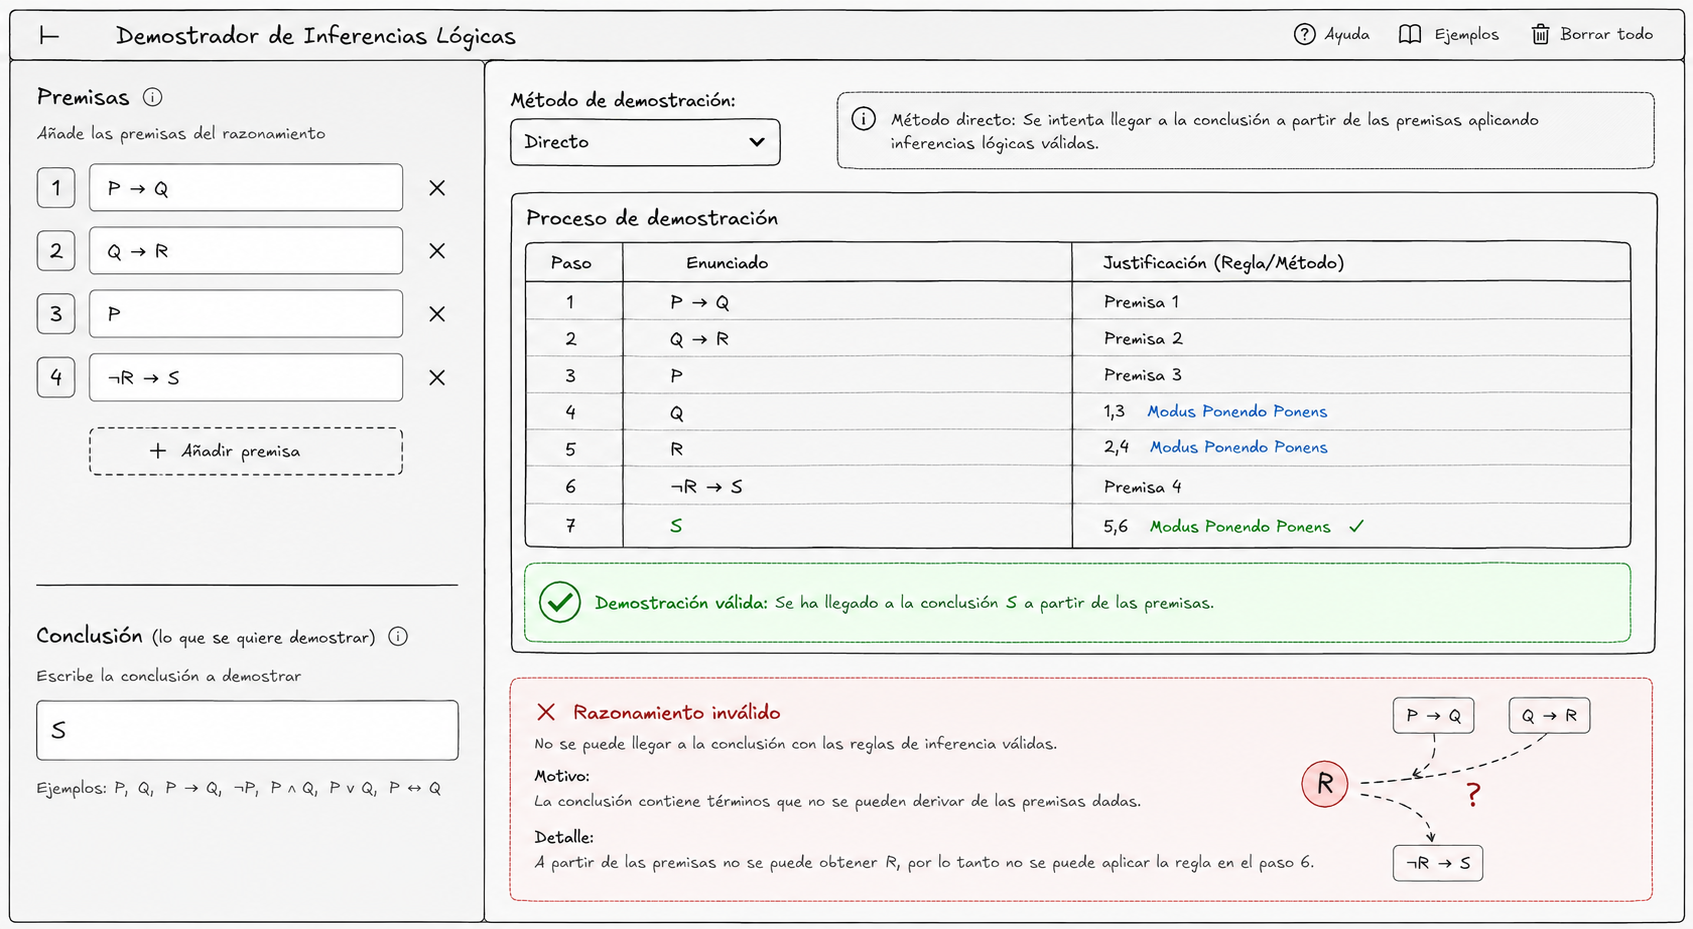
\includegraphics[width=0.82\textwidth,keepaspectratio]{propuesta-arnold.png}
    \caption{Boceto preliminar (Wireframe) del Módulo 1: Resolución y Demostración Automática.}
\end{figure}

\begin{figure}[h!]
    \centering
    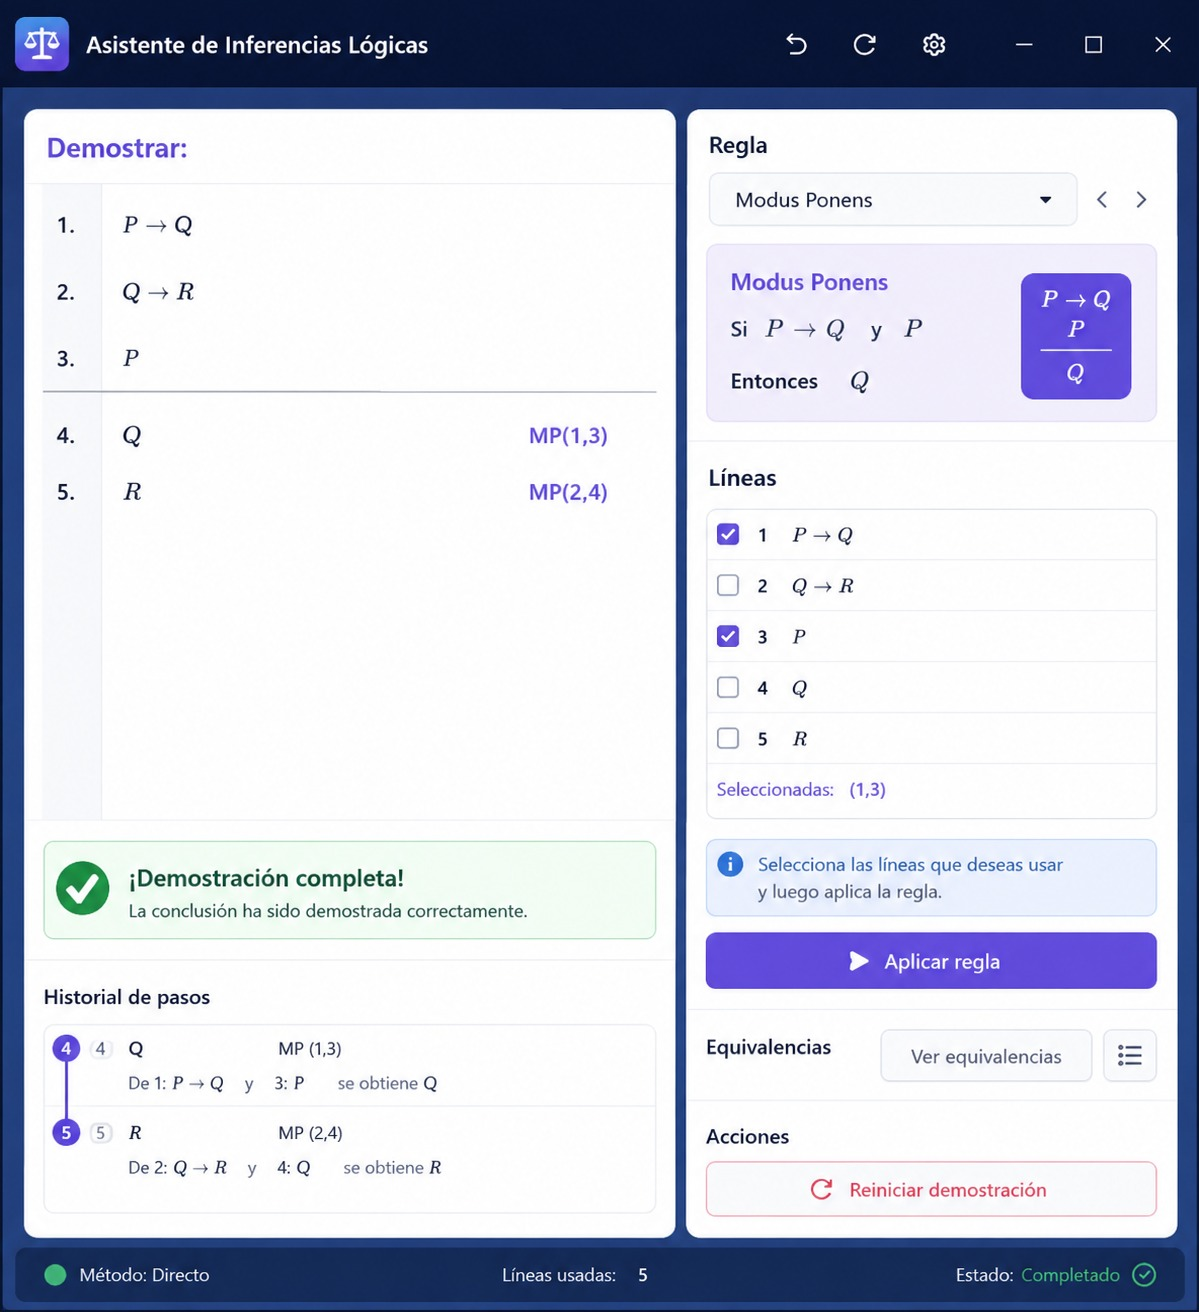
\includegraphics[width=0.82\textwidth,keepaspectratio]{propuesta-morocho.jpeg}
    \caption{Boceto preliminar (Wireframe) del Módulo 2: Entorno de Práctica Interactiva y Validación.}
\end{figure}

\begin{figure}[h!]
    \centering
    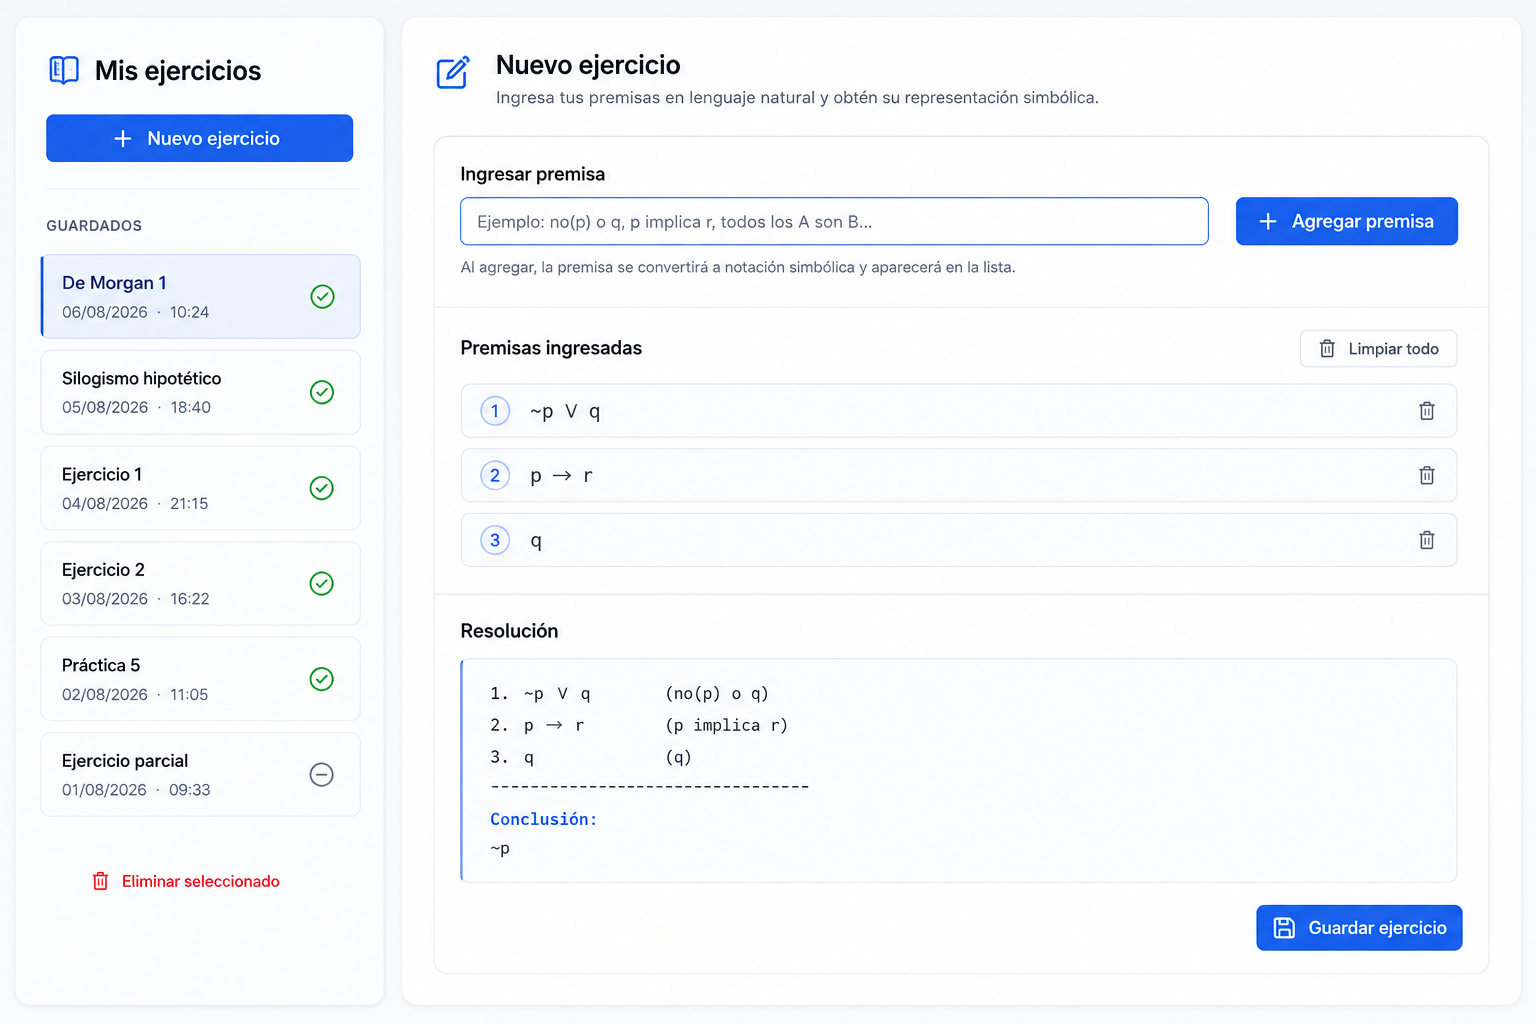
\includegraphics[width=0.82\textwidth,keepaspectratio]{propuesta-alex.png}
    \caption{Diseño y maquetación de la propuesta visual integrada para el sistema de inferencias.}
\end{figure}

% =========================================================================
% SECCIÓN 2: ARQUITECTURA Y GIT FLOW
% =========================================================================
\newpage
\section{Arquitectura del Software y Flujo de Trabajo (Git Flow)}

El proyecto fue desarrollado bajo una \textbf{arquitectura modular y desacoplada}, asegurando que la lógica computacional del motor de inferencias no posea dependencia alguna respecto al framework de presentación visual.

\subsection{Estructura de Directorios del Módulo}
La organización física del código fuente se divide claramente entre la capa matemática pura y la capa de componentes reactivos:

\begin{itemize}[leftmargin=1.2cm]
    \item \textbf{Capa Lógica y Motor Matemático (\texttt{src/lib/}):}
    \begin{itemize}
        \item \texttt{src/lib/solver/types.ts}: Definición formal de los tipos del Árbol de Sintaxis Abstracta (AST), operadores lógicos, reglas y modelos de contraejemplo.
        \item \texttt{src/lib/solver/parser.ts}: Tokenizador léxico y analizador sintáctico por descenso recursivo con precedencia de operadores.
        \item \texttt{src/lib/solver/solver.ts}: Algoritmo de \textit{Forward Chaining}, evaluador semántico de verdad ($2^N$), detector de falacias y aplicación de 11 reglas de deducción natural.
        \item \texttt{src/lib/validator/validator.ts}: Sanitizador de cadenas, normalización de notaciones heterogéneas y validador reactivo sin excepciones.
        \item \texttt{src/lib/trazabilidad/historial.ts}: Gestor de historial de deducción, numeración de pasos y resolución de referencias cruzadas.
        \item \texttt{src/lib/transcription/descriptionGenerator.ts} y \texttt{naturalTranslator.ts}: Generación de explicaciones semánticas en español y traducción de variables a argumentos continuos.
    \end{itemize}
    \item \textbf{Capa de Interfaz de Usuario (\texttt{src/pages/inferencias/} y \texttt{src/components/inferencias/}):}
    \begin{itemize}
        \item \texttt{index.vue}: Orquestador reactivo principal con teclado virtual y pestañas de modo formal vs. lenguaje natural.
        \item \texttt{FormularioInferencia.vue}: Captura dinámica de premisas, teclado asistido y validación visual.
        \item \texttt{IndicadorResultado.vue}: Semáforo visual de 3 estados con diagnóstico explícito de falacias.
        \item \texttt{PanelTrazabilidad.vue}: Tabla formal numerada $(1), (2), \dots \therefore (N)$, acordeón explicativo y exportadores a \LaTeX\ y Markdown.
        \item \texttt{TraductorLenguajeNatural.vue}: Asignación contextual de proposiciones cotidianas.
    \end{itemize}
    \item \textbf{Documentación y Tareas de Sprint (\texttt{TAREAS/}):}
    \begin{itemize}
        \item \texttt{TAREAS/01\_Propuesta/hijos-de-linus/propuesta.md}: Documento de propuesta inicial y bocetos.
        \item \texttt{TAREAS/02\_Motor/hijos-de-linus/avance.md} y \texttt{casos\_de\_prueba.md}: Avances del motor y matriz de 25 casos límite.
        \item \texttt{TAREAS/03\_UI/hijos-de-linus/avance.md} y \texttt{glosario-diseno.md}: Avance de componentes y guía de diseño.
        \item \texttt{TAREAS/04\_Deploy/hijos-de-linus/uso.md} y \texttt{errores\_y\_soluciones.md}: Manual de uso y reporte de control de calidad.
    \end{itemize}
\end{itemize}

\subsection{Flujo de Git por Ramas (Git Flow)}
Para garantizar la estabilidad del repositorio compartido con los demás equipos, se utilizó un flujo estricto de integración continua basado en ramas por sprint y Pull Requests atómicos:

\begin{itemize}[leftmargin=1.2cm]
    \item \texttt{sprint-1-propuesta}: Maquetación, definición de requerimientos y casos de uso iniciales.
    \item \texttt{sprint-2-hijos-de-linus}: Implementación del AST, Parser, Solver, Validador, Trazabilidad y pruebas unitarias de motor.
    \item \texttt{sprint-3-hijos-de-linus}: Construcción de los 4 componentes Vue 3, teclado simbólico e integración de la vista.
    \item \texttt{sprint-3.5-fase-inicial}: Incorporación de diagnósticos con contraejemplos, acordeón didáctico y exportación \LaTeX.
    \item \texttt{deploy / main}: Fusión final validada con 113 pruebas automáticas y 0 errores de tipado en TypeScript.
\end{itemize}

% =========================================================================
% SECCIÓN 3: CAPA LÓGICA (SPRINT 2)
% =========================================================================
\newpage
\section{Capa Lógica: El Motor de Inferencia y Demostración (Sprint 2)}

El motor computacional de inferencias lógicas opera mediante un pipeline determinista de cuatro fases:

\begin{enumerate}[label=\textbf{Fase \arabic*:}]
    \item \textbf{Sanitización y Normalización Léxica:}
    Unifica las múltiples notaciones matemáticas y lógicas ingresadas por el estudiante (\texttt{->}, \texttt{∧}, \texttt{∨}, \texttt{¬}, \texttt{\~}, \texttt{\&}, \texttt{|}, \texttt{⊕}, \texttt{△}, \texttt{↔}) convirtiéndolas en identificadores estándar (\texttt{ENTONCES}, \texttt{Y}, \texttt{O}, \texttt{NO}, \texttt{O\_EXCLUSIVA}, \texttt{SI\_Y\_SOLO\_SI}), eliminando caracteres inválidos y previniendo inyecciones de código.

    \item \textbf{Analizador Sintáctico (Parser AST por Descenso Recursivo):}
    Convierte la secuencia lineal de tokens en un Árbol de Sintaxis Abstracta estructurado, respetando la jerarquía y precedencia matemática rigurosa:
    $$\text{Negación } (\neg) \quad > \quad \text{Conjunción } (\land) \quad > \quad \text{Disyunciones } (\lor, \triangle) \quad > \quad \text{Condicional } (\to) \quad > \quad \text{Bicondicional } (\leftrightarrow)$$

    \item \textbf{Motor Deductivo (Forward Chaining y Pattern Matching):}
    Aplica de manera iterativa (hasta 12 niveles de derivación) las 11 reglas clásicas de deducción natural:
    \begin{itemize}[leftmargin=0.8cm]
        \item \textbf{Modus Ponendo Ponens (MPP):} $A \to B, \, A \vdash B$
        \item \textbf{Modus Tollendo Tollens (MTT):} $A \to B, \, \neg B \vdash \neg A$
        \item \textbf{Silogismo Disyuntivo (SD):} $A \lor B, \, \neg A \vdash B \quad / \quad A \lor B, \, \neg B \vdash A$
        \item \textbf{Silogismo Disyuntivo Exclusivo (SDE):} $A \triangle B, \, A \vdash \neg B \quad / \quad A \triangle B, \, B \vdash \neg A$
        \item \textbf{Silogismo Hipotético (SH):} $A \to B, \, B \to C \vdash A \to C$
        \item \textbf{Simplificación y Conjunción:} $A \land B \vdash A, \, B \quad / \quad A, \, B \vdash A \land B$
        \item \textbf{Dilema Constructivo (DC):} $(A \to B) \land (C \to D), \, A \lor C \vdash B \lor D$
        \item \textbf{Bicondicionales:} Modus Ponens Bicondicional y Eliminación Bicondicional ($A \leftrightarrow B \vdash A \to B, \, B \to A$).
    \end{itemize}

    \item \textbf{Evaluador Semántico SAT ($2^N$ combinaciones de verdad):}
    Garantiza la clasificación estricta del razonamiento en 3 estados de validez:
    \begin{itemize}
        \item \textbf{Inferencia Válida (Demostrada):} Se completó la deducción paso a paso mediante reglas directas.
        \item \textbf{Inferencia Válida (Método Indirecto Requerido):} El argumento es lógicamente válido ($0$ contraejemplos semánticos), pero requiere Reducción al Absurdo o Prueba Condicional.
        \item \textbf{Inferencia Inválida (Refutada por Contraejemplo):} Detecta la asignación concreta donde todas las premisas son verdaderas y la conclusión es falsa, diagnosticando falacias como el Dilema Inverso o Afirmación del Consecuente.
    \end{itemize}
\end{enumerate}

\subsection{Código Fuente del Motor Lógico}
A continuación, se detalla el evaluador semántico y la detección de modelos implementados en \texttt{src/lib/solver/solver.ts}:

\begin{lstlisting}[caption={Evaluador semántico AST y detección de contraejemplos (solver.ts).}]
// src/lib/solver/solver.ts
export function evaluarNodo(
  nodo: NodoExpresion,
  asignacion: Record<string, boolean>
): boolean {
  if (nodo.tipo === 'variable') {
    return Boolean(asignacion[nodo.nombre.toUpperCase()]);
  }
  if (nodo.tipo === 'operacion') {
    if (nodo.operador === 'NO' && nodo.derecho) {
      return !evaluarNodo(nodo.derecho, asignacion);
    }
    if (nodo.izquierdo && nodo.derecho) {
      const izq = evaluarNodo(nodo.izquierdo, asignacion);
      const der = evaluarNodo(nodo.derecho, asignacion);
      switch (nodo.operador) {
        case 'Y': return izq && der;
        case 'O': return izq || der;
        case 'O_EXCLUSIVA': return izq !== der; // Disyuncion fuerte
        case 'ENTONCES': return !izq || der;
        case 'SI_Y_SOLO_SI': return izq === der;
        case 'NI': return !(izq || der);
        case 'INCOMPATIBLE': return !(izq && der);
        default: return false;
      }
    }
  }
  return false;
}
\end{lstlisting}

% =========================================================================
% SECCIÓN 4: CAPA VISUAL (SPRINT 3 Y 3.5)
% =========================================================================
\newpage
\section{Capa Visual: Interfaz Reactiva y Didáctica (Sprint 3 y 3.5)}

La interfaz gráfica (\texttt{src/pages/inferencias/index.vue}) fue construida bajo la guía de diseño del proyecto, priorizando claridad visual, respuesta reactiva instantánea y accesibilidad universal.

\subsection{Reactividad en Vue 3 y Composition API}
\begin{itemize}[leftmargin=1.2cm]
    \item \textbf{Flujo Reactivo Unidireccional:} Empleo estricto de \texttt{ref}, \texttt{computed} y tipado mediante interfaces compartidas (\texttt{src/types/inferencias.ts}), evitando estados globales superfluos.
    \item \textbf{Teclado Simbólico en Pantalla:} Permite insertar conectivos lógicos ($\neg$, $\land$, $\lor$, $\triangle$, $\to$, $\leftrightarrow$, $($, $)$) con un solo clic o toque en dispositivos móviles, manteniendo la posición del cursor en el input activo.
    \item \textbf{Pestañas de Visualización:} Permite conmutar instantáneamente entre el formato de \textit{Simbología Formal} y el de \textit{Lenguaje Natural}, sincronizando en tiempo real las variables proposicionales.
\end{itemize}

\subsection{Trazabilidad Pedagógica y Herramientas Académicas}
\begin{itemize}[leftmargin=1.2cm]
    \item \textbf{Desglose Particionado con Acordeón Colapsable:} Cada paso de la demostración formal incluye un botón interactivo (\textit{¿Por qué esta regla?}) que despliega:
    \begin{itemize}
        \item Las líneas de premisa base utilizadas y su rol deductivo (ej. \textit{Condicional base}, \textit{Antecedente afirmado}).
        \item La regla formal aplicada y su justificación semántica en español.
        \item La conclusión parcial derivada.
    \end{itemize}
    \item \textbf{Exportación en 1 Clic a \LaTeX\ y Markdown:} Formatea automáticamente la demostración completa en código compatible con artículos científicos:
    $$\begin{aligned}
        (1) \quad & P \to Q && \text{(Premisa)} \\
        (2) \quad & P && \text{(Premisa)} \\
        \therefore (3) \quad & Q && \text{(Modus Ponendo Ponens de 1, 2)}
    \end{aligned}$$
    \item \textbf{Historial Persistente en Memoria Local (\texttt{localStorage}):} Almacena las últimas demostraciones realizadas para permitir su restauración inmediata.
\end{itemize}

% =========================================================================
% SECCIÓN 5: PRUEBAS DE CALIDAD (SPRINT 4)
% =========================================================================
\section{Pruebas de Calidad del Código (Sprint 4)}

Para certificar la confiabilidad matemática del software, se implementó una suite de pruebas automatizadas con \textbf{Vitest}:

\begin{itemize}[leftmargin=1.2cm]
    \item \textbf{Cobertura Exhaustiva:} \textbf{13 archivos de prueba y 113 tests unitarios e integrados} ejecutados con 100\% de éxito.
    \item \textbf{Chequeo Estricto de Tipos:} Verificación continua con \texttt{vue-tsc -{}-noEmit} (\textbf{0 errores de TypeScript}).
    \item \textbf{Pruebas de Estrés y Seguridad (\textit{Fuzzer}):} Evaluación de expresiones con hasta 10 niveles de anidación, caracteres corruptos, emojis y mitigación de inyecciones de código malicioso.
    \item \textbf{Validación de Casos Límite:} Pruebas de derivación encadenada de hasta 6 pasos, disyunción exclusiva fuerte y contraejemplos matemáticos precisos.
\end{itemize}

\vspace{0.2cm}
\begin{tcolorbox}[colback=lightbg,colframe=accentblue,arc=2mm,title=\textbf{Resultados de la Suite de Pruebas (Vitest)}]
\texttt{✓ src/lib/solver/solver.test.ts (15 tests)}\\
\texttt{✓ src/lib/solver/parser.test.ts (12 tests)}\\
\texttt{✓ src/lib/validator/validator.test.ts (27 tests)}\\
\texttt{✓ src/lib/validator/validator\_stress.test.ts (15 tests)}\\
\texttt{✓ src/lib/trazabilidad/trazabilidad.test.ts (9 tests)}\\
\texttt{✓ src/lib/integracion\_motor.test.ts (8 tests)}\\
\texttt{✓ src/components/inferencias/\_\_tests\_\_/* (27 tests)}\\
\textbf{\textcolor{commentgreen}{Total: 13 archivos pasados (13) | 113 tests pasados (113) — 100\% Éxito}}
\end{tcolorbox}

% =========================================================================
% SECCIÓN 6: PARTICIPACIÓN Y APORTES
% =========================================================================
\newpage
\section{Participación y Aportes del Equipo}

La asignación de responsabilidades entre los integrantes del \textbf{Equipo Los Hijos de Linus} se resume en la Tabla 1:

\vspace{0.4cm}
\begin{table}[h!]
\centering
\small
\renewcommand{\arraystretch}{1.35}
\begin{tabularx}{\textwidth}{|>{\bfseries}p{4.5cm}|>{\raggedright\arraybackslash}p{3.8cm}|>{\raggedright\arraybackslash}X|}
\hline
\rowcolor{headerblue}
\textcolor{white}{Integrante} & \textcolor{white}{Rol Principal} & \textcolor{white}{Contribución Clave} \\
\hline
Altamirano Astupiñan, Renatto André & Ingeniero de Pruebas y Calidad (QA) & Implementación del validador y sanitizador (\texttt{validator.ts}), diseño de matriz de 25 casos límite, tests de estrés (\textit{fuzzer}) y configuración de Vitest. \\
\hline
Centurión Gonzales, Alex & Desarrollador Frontend y UX & Implementación de \texttt{IndicadorResultado.vue}, semáforo de 3 estados, diseño del acordeón didáctico de trazabilidad y feedback visual de falacias. \\
\hline
Espinoza Orrego, Piero Arom & Arquitecto de Software y Motor Lógico & Modelado del AST, analizador léxico y sintáctico por descenso recursivo (\texttt{parser.ts}), motor de \textit{Forward Chaining} (\texttt{solver.ts}) e integración global de la vista. \\
\hline
Mio Caballero, Arnold André & Ingeniero de Transcripción y Lenguaje Natural & Desarrollo del generador de explicaciones didácticas (\texttt{translations.ts}, \texttt{descriptionGenerator.ts}), renderizador de AST y componente \texttt{TraductorLenguajeNatural.vue}. \\
\hline
Morocho Lumbre, Juan David & Analista de Lógica y Trazabilidad & Construcción del contenedor de historial y trazabilidad (\texttt{historial.ts}), algoritmo de diagnóstico de errores lógicos (\textit{pattern matching}) y desarrollo de \texttt{FormularioInferencia.vue}. \\
\hline
\end{tabularx}
\caption{Distribución de roles y contribuciones técnicas del equipo.}
\end{table}

% =========================================================================
% SECCIÓN 7: TRABAJO EN EQUIPO
% =========================================================================
\section{Trabajo en Equipo}

El desarrollo del proyecto se articuló mediante sesiones de trabajo colaborativo en la plataforma \textbf{Google Meet}, las cuales sirvieron como espacio centralizado para la coordinación técnica, revisión de código en vivo y planificación iterativa de cada sprint.

La metodología colaborativa contempló:
\begin{itemize}[leftmargin=1.2cm]
    \item \textbf{Pair Programming y Code Review:} Validación de componentes y funciones críticas antes de fusionar Pull Requests.
    \item \textbf{Sincronización Continua con Git Flow:} Manejo disciplinado de ramas por sprint, asegurando commits atómicos y evitando conflictos con los otros equipos del repositorio.
    \item \textbf{Cultura de Calidad:} Comprobación sistemática de tipado (\texttt{npm run type-check}) y ejecución de pruebas unitarias antes de cada entrega.
\end{itemize}

% =========================================================================
% SECCIÓN 8: CONCLUSIONES
% =========================================================================
\section{Conclusiones}

\begin{enumerate}[label=\textbf{\arabic*.}]
    \item \textbf{Innovación Pedagógica en la Enseñanza de la Lógica:} Se construyó una plataforma web capaz de convertir la demostración formal de inferencias en un proceso didáctico transparente, combinando derivaciones formales con justificaciones en lenguaje natural y contraejemplos matemáticos claros.
    \item \textbf{Arquitectura Limpia, Modular y Escalable:} La separación estricta entre la biblioteca matemática en TypeScript puro (\texttt{src/lib/}) y la capa de presentación en Vue 3 (\texttt{src/components/}) garantizó alta cohesión, bajo acoplamiento y facilitó un flujo de trabajo paralelo sin interferencias.
    \item \textbf{Rigor Matemático y Verificación Exhaustiva:} La combinación del motor deductivo de \textit{Forward Chaining} con el evaluador semántico SAT de $2^N$ combinaciones permitió resolver con precisión absoluta los 3 estados de validez del argumento, alcanzando 100\% de aprobación en la suite de 113 pruebas automatizadas.
\end{enumerate}

\end{document}
